% Toy Model
\section{Stochastic toy landscape}
\label{sec:toy_model}

\subsection{Landscape potential}

The landscape is a one-dimensional field $\phi$ with a quadratic base potential
$V_0(\phi) = \frac12 m^2 \phi^2$ ($m^2 = 0.1$) plus six Gaussian well
perturbations at positions $\mu \in \{-4.0, -1.5, 0.5, 2.5, 4.0, 6.0\}$
with depths $V_0(\mu)$ scaled to produce distinct basin minima.
Fig.~\ref{fig:landscape} shows the potential and basin labels.

\begin{figure}[t]
  \centering
  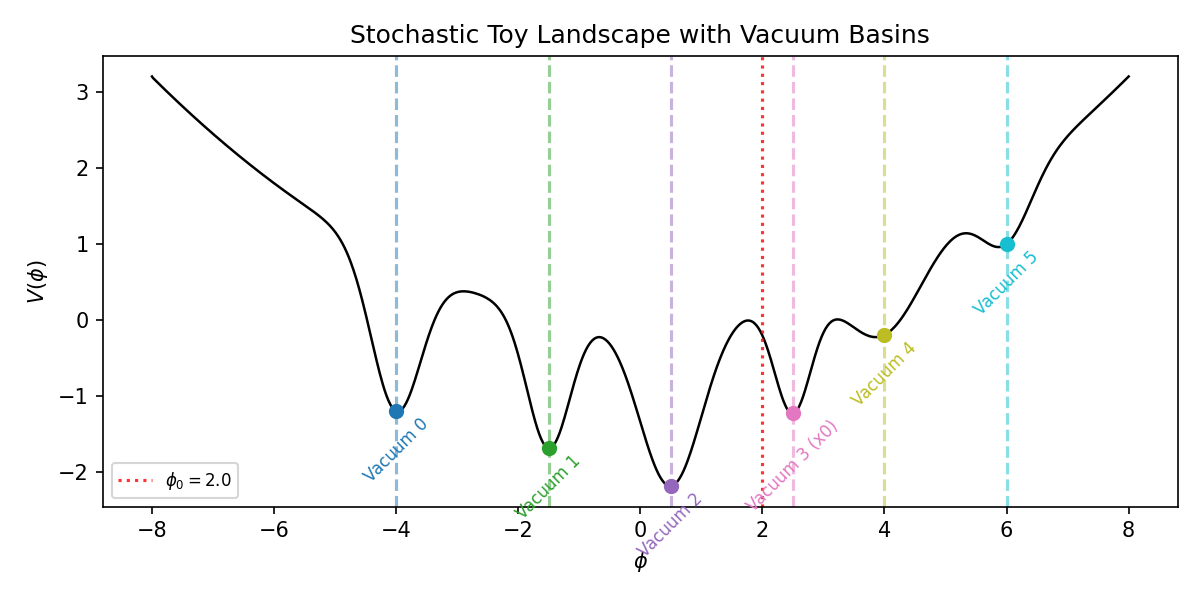
\includegraphics[width=\columnwidth]{figures/fig_01_landscape_basins.png}
  \caption{Stochastic toy landscape $V(\phi)$ with six vacuum basins.
  The observable patch $\phi_0 = 2.0$ (red dotted line) lies in basin~3.
  Each basin is assigned an effective physics vector $\boldsymbol{\theta}$.}
  \label{fig:landscape}
\end{figure}

\subsection{Basin assignment}

Each well center defines a vacuum basin.
Basin identity is determined by the nearest local minimum of the potential.
The observable patch at $\phi_0 = 2.0$ is identified with basin~3 via
\verb|landscape.identify_basin(phi0)|, not from the first sampled trajectory.
This matters for the stress test, where the first trajectory can land in any basin.

\subsection{Initial conditions and dynamics}

Initial field values are sampled from a normal distribution
$\phi_{\rm init} \sim \mathcal{N}(\phi_0, \sigma^2)$ with $\sigma = 1.5$
by default.
Each trajectory evolves via a Langevin-like stochastic differential equation
over 80~$e$-folds with time step $\Delta t = 0.1$.
The main run uses $N = 10,\!000$ trajectories; stress tests use $N = 2,\!000$.

\subsection{Effective physics vector}

Each basin $v$ is assigned a physics vector
$\boldsymbol{\theta}(v) = (\Lambda_{\rm eff}, G_{\rm eff}, Q_{\rm fluct}, T_{\rm reh})$
with toy values reflecting different phenomenological profiles.
These values are arbitrary placeholders; they demonstrate the mechanism
of unobserved-sector reweighting but carry no claim about real cosmology.

\subsection{Cutoff list}

We evaluate measures at cutoffs
$N_k \in \{100, 250, 500, 1000, 2500, 5000, 10000\}$.
Cutoffs exceeding the total number of sectors are dropped.
